\chapter{React Native} \label{chapter:reactnative}
In maart 2015 bracht Facebook het open-source framework React Native uit voor iOS. React Native is sinds maart verkrijgbaar via GitHub en kan genieten van een hoge populariteit bij ontwikkelaars. Toen Facebook in maart het nieuws openbaar maakte, werd het Android gedeelte van de app met een vertraging van 6maanden aangekondigd. Op 14 september was het dan zo ver, React Native kan nu ook gebruikt worden om Android applicaties te schrijven op de React manier. 
\centerline{
	\begin{minipage}{.8\linewidth}
		\vspace*{2ex}
		\emph{``React Native brings what developers are used to from React on the Web -- declarative self-contained UI components and fast development cycles -- to the mobile platform, while retaining the speed, fidelity and feel of native applications.’’}
		\\ \hspace*{1pt}\hfill --- 
		\citep{Witte:React}
		\vspace*{2ex}
	\end{minipage}
}

De aanpak van Facebook om applicaties te schrijven in JavaScript is niet nieuw maar React Native heeft een heel eigen manier ontwikkeld om dit te kunnen realiseren.
\section{Native applicatie}
Een native applicatie is een applicatie die ontwikkeld is voor een specifiek platform. De maker van het platform heeft hiervoor een specifieke programmeertaal aangeduid, met API om de platform specifieke componenten, views, enz.. te kunnen gebruiken. Vaak zijn hieraan ook duidelijke en verplichte richtlijnen aan verbonden om te mogen/kunnen programmeren voor dit specifieke platform. De applicaties worden verkrijgbaar gemaakt in stores die door de aanbieders van het OS worden aangeboden.

Positieve eigenschappen van native ontwikkeling : 
\begin{itemize}
\item Er kan maximaal gebruik gemaakt worden van alle beschikbare functionaliteiten van het apparaat waarop de applicatie draait.
\item Een native applicatie heeft toegang tot de bibliotheek voor het gebruik van media.
\item Het is niet noodzakelijk om met het internet verbonden te zijn.
\item Een native applicatie heeft een snelle en gebruiksvriendelijke UX.
\end{itemize}
Toch zijn er ook negatieve eigenschappen aan verbonden : 
\begin{itemize}
\item De applicatie moet ontwikkeld worden op elk platform afzonderlijk.
\item Er is een goedkeuring nodig om de applicatie te publiceren in de applicatie stores.
\item Een update in de software van de OS betekend vaak dat een applicatie moet aangepast worden.
\item Hoge ontwikkelingskost.
\end{itemize}

Op niveau van mobiele applicaties zijn er verschillende OS, dit zijn de belangrijkste en meest voorkomende : 
\begin{itemize}
\item \textbf{Android} : ontwikkeld door Google.
\item \textbf{iOS} : ontwikkeld door Apple.
\item \textbf{Windows Phone} : ontwikkeld door Microsoft.
\item \textbf{BlackBerry OS} : ontwikkeld door RIM (Research In Motion).
\item Symbian, Java ME, Kindle, Bada, ... 
\end{itemize}

Android en iOS hebben volgens IDC (International Data Corporation)(\prettyref{fig:idc}) samen een marktaandeel van 96.7\%. Windows phone is daarna de grootste met slechts 2.6\%. \citep{idc:mobile}

	\begin{figure}
		\centering
		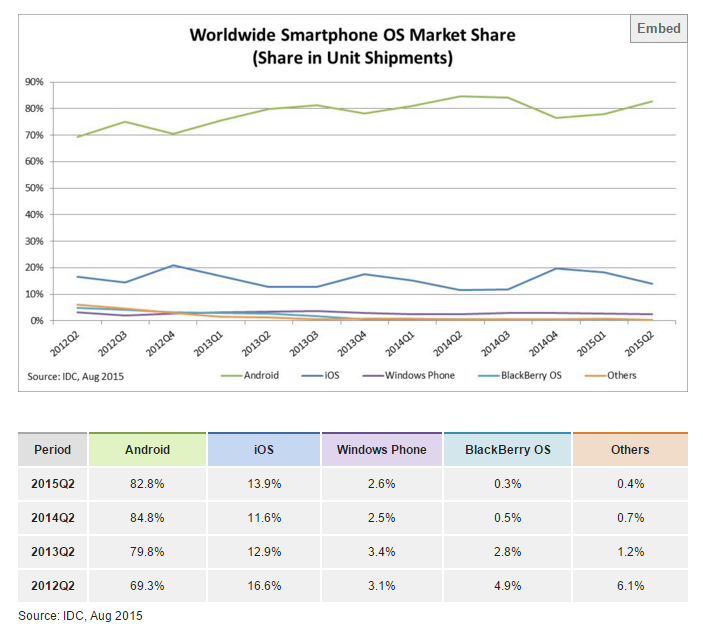
\includegraphics[width=.5\columnwidth]{img/idc.png}
		\caption{IDC - worldwide smartphone OS Market Share, Aug 2015}
		\label{fig:idc}
	\end{figure}

\section{Hybride applicaties}\label{section:hybride}

Hybride applicaties zijn een combinatie van een native component, vaak een webview, en een web applicatie in HTML en JavaScript. Deze aanpak wordt weleens de “best of both worlds” -aanpak genoemd omdat ze de voordelen van een native applicatie combineren met de voordelen van een web applicatie, en het grootste voordeel is natuurlijk dat de code slechts één keer geschreven hoeft te worden. Bij een hybride applicatie is het dus meestal zo dat de ontwikkelaar de applicatie gaat programmeren zoals een web applicatie maar deze wordt als het ware gewrapt in een native webview component van het specifieke platform waarvoor de applicatie bedoeld wordt. 
Wanneer een ontwikkelaar de native API componenten, zoals camera, gebruikerslocatie, … wenst te gebruiken in zijn applicatie dan kan die daarvoor gebruik maken van een framework zoals PhoneGap, Ionic of Cordova. Deze frameworks maken gebruik van HTML5, CSS en JavaScript om hybride applicaties voor mobiel te ontwikkelen.

Positieve eigenschappen van hybride applicaties : 
\begin{itemize}
	\item Een hybride applicatie moet slechts éénmaal geschreven worden om op verschillende platformen te kunnen draaien. \prettyref{fig:hybridevsnative}
	\item Een hybride applicatie heeft mogelijkheden om native componenten te gebruiken.
	\item De inhoud van een hybride applicatie kan snel ge-update worden.
	\item Hybride applicaties kunnen in de stores geplaatst worden.
	\item De ontwikkelingskost voor een hybride applicatie is minder dan die van een native applicatie.
\end{itemize}
Negatieve eigenschappen van hybride applicaties : 
\begin{itemize}
	\item De ontwikkelaar heeft een brede kennis nodig, zowel web als native kennis zijn vereist.
	\item Hybride applicaties zijn niet geschikt voor games of zware grafische applicaties.
	\item Een hybride applicatie loopt over het algemeen trager dan een native applicatie.
	\item Een hybride applicatie is niet altijd offline beschikbaar.
\end{itemize}
De populariteit van hybride applicaties groeit en de voordelen zijn voor vele applicatie ontwikkelaars een doorslaggevend argument om te kiezen voor een hybride oplossing. Toch moeten ontwikkelaars telkens afwegen hoe men de applicatie zal ontwikkelen, hybride of native. De vraag die telkens gesteld moet worden is hoe een applicatie de beste gebruikerservaring kan bekomen.

Een aantal voorbeelden van populaire hybride applicaties : 

\begin{itemize}
	\item \textbf{Uber} : applicatie voor een soort taxiservice.
	\item \textbf{Apple's app store} : Apple heeft zijn liefde voor HTML5 nooit onder stoelen of banken gestoken, en de appstore is inderdaad een hybride applicatie.
	\item \textbf{Twitter} : sociaal netwerk applicatie.
\end{itemize}

Uit deze voorbeelden kan de conclusie getrokken worden dat wanneer men een applicatie wenst te bouwen die veel http aanvragen (post, get, ….) zal moeten uitvoeren, best hybride ontwikkeld wordt.
	
	\begin{figure}
		\centering
		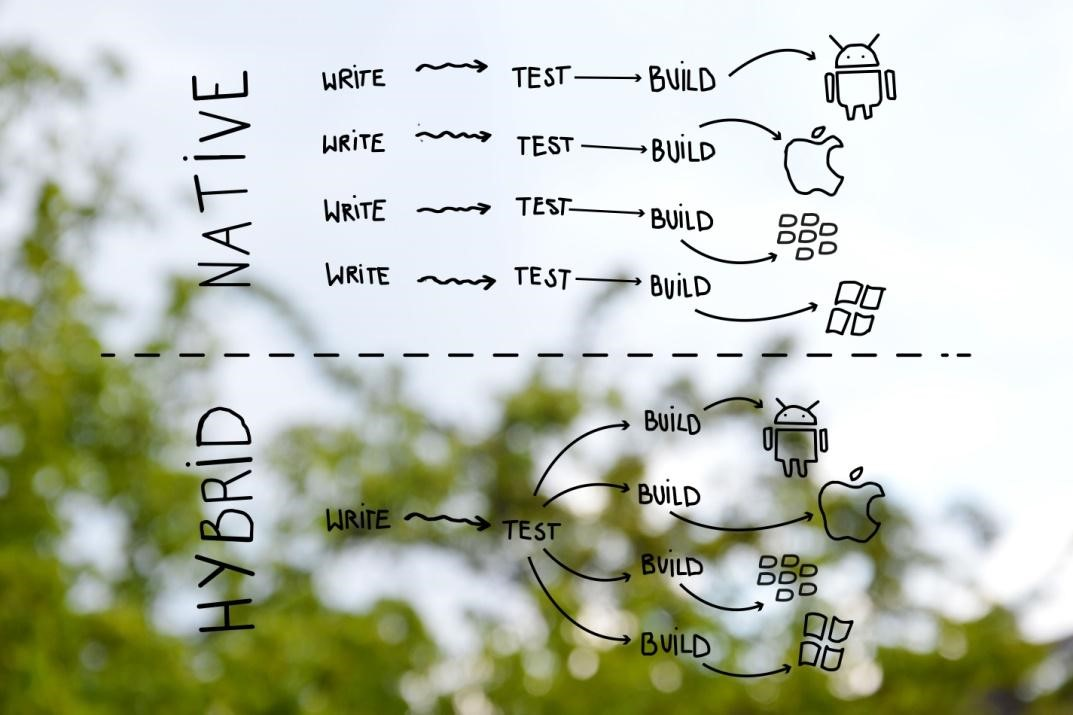
\includegraphics[width=.5\columnwidth]{img/hybridevsnative.jpg}
		\caption{Hybride vs. Native write-test-build}
		\label{fig:hybridevsnative}
	\end{figure}
	
	\section{Waarom React Native?}
	Er zijn verschillende redenen waarom native mobiele omgevingen moeilijker zijn om mee te werken dan het web. Allereerst, is het moeilijk om componenten weer te geven op het scherm, deze moeten vaak manueel op de view geplaatst worden en ze moeten voorzien worden van een grootte. Daarnaast was er geen mogelijkheid om React code te integreren, die het proces voor bouwen van websites met telkens veranderende datasets had vereenvoudigd. 
	
De grootste ergernis bij Facebook ingenieurs was dat wanneer er native applicaties werden gebouwd ze rekening moesten houden met het telkens heropstarten van de applicatie wanneer er iets werd gewijzigd. De wijzigingen van een knop die aantal centimeter werd verplaatst, bijvoorbeeld zorgde ervoor dat als men de wijziging op het scherm wou weergeven de applicatie volledig herstart moest worden. Wat het ontwikkelingsproces sterk vertraagde. 
Bij Facebook wordt er 2 maal per dag (!) een nieuwe versie van de website afgeleverd zodat resultaten van een bepaald experiment onmiddellijk worden waargenomen en eventuele fouten per direct kunnen worden opgelost. Bij de native applicatie van Facebook moet er vaak weken of maanden gewacht worden om een wijziging te kunnen doorvoeren, omdat de aanbieders van de stores deze eerst moeten nakijken en goedkeuren. Dit brengt een hoop tijdsverlies  en dus ook geldverlies met zich mee. 

``Move fast'' zit bij Facebook in het DNA, maar men was gebonden aan de regels van de mobiele OS aanbieders om de wijzigingen van hun applicaties te kunnen doorvoeren. Toch wou men bij Facebook niet inbinden op de gebruikerservaring en het uitzicht van de applicatie, deze moesten native blijven. \citep{occhino:React}

\section{Wat is React Native?}
React Native is een JavaScript framework die gebruik maakt van de React library, om native applicaties voor iOS (iPhone, iPad) en Android te schrijven, hierdoor kunnen ze het grootste deel van de smartphone en tablet gebruikers bereiken. Toch gebruikt Facebook in React Native een hybride aanpak, want het maakt gebruik van JavaScript maar de applicatie zal volledig native beschouwd worden.

Dankzij dit framework heeft Facebook het mogelijk gemaakt voor web ontwikkelaars om applicaties te schrijven voor mobiele platformen in de reeds beheerste JavaScript taal en omdat het grootste deel van de code gedeeld kan worden tussen beide platformen wordt een gekend probleem van mobiele applicatie ontwikkeling geëlimineerd, nl. dat eenzelfde applicatie in meerdere programmeer talen geschreven moest worden. 

Net zoals React worden React Native applicaties geschreven in een mix van JavaScript en JSX. Onderliggend is er een soort brug voorzien die de componenten van de API’s in Objective C (iOS) of Java (Android) gaan aanspreken en gebruiken in de applicatie. Met andere woorden, de applicaties die gemaakt worden in React Native maken gebruik van echte mobiele UI componenten, en geen webviews zoals vele hybride applicaties, zodat de applicatie aanvoelt voor de gebruiker zoals elke andere mobile applicatie geschreven in de native taal. Daarnaast zijn er ook interfaces voorzien die de hardware componenten zoals camera, gebruikerslocatie, … kunnen aanspreken.

\section{Hoe werkt React Native?}
Om de werking van React Native te kunnen begrijpen moet de werking van React gekend zijn, nl. de manier waarop React omgaat met het virtuele DOM (\prettyref{section:virtualdom}). React plaatst zoals eerder vermeld een abstractie laag tussen de code van de ontwikkelaar en hetgeen dat zichtbaar is voor de gebruiker. Maar wanneer gesproken wordt over native mobiele applicaties dan wordt er niet gewerkt met de browser, en moest Facebook een andere oplossing zoeken om deze manier van werken ook te kunnen toepassen. 

Facebook heeft hiervoor met React Native een gepaste oplossing bedacht, in plaats van gebruik te maken van het DOM van de browser gaat React Native Objective C API’s gebruiken om iOS componenten weer te geven, of Java API’s gebruiken om Android componenten weer te geven.  In \prettyref{fig:dombridge} wordt het verschil tussen een React component en React Native component op gebied van weergave getoond. In plaats van het Virtuele DOM wordt de “bridge” aangesproken om de juiste weergave te tonen in de juiste OS.  

	\begin{figure}
		\centering
		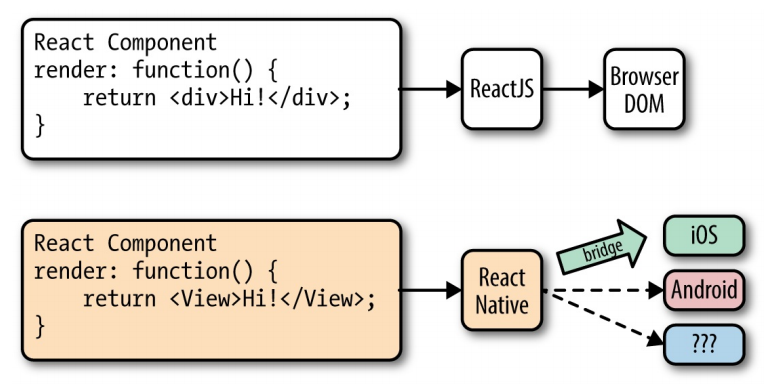
\includegraphics[width=\columnwidth]{img/bridge.png}
		\caption{Virtual DOM vs bridge}
		\label{fig:dombridge}
	\end{figure}


De bridge of brug die gemaakt wordt voorziet React van een interface in de platform specifieke UI elementen. De layout die voorzien wordt door de render functie van een React component zal met ander woorden vertaald worden naar een gepaste component. Bv. <view> kan vertaald worden naar een iOS specifieke UIView. De brug is niet uniek aan React, het PhoneGap framework gebruikt ook een brug om API’s aan te spreken, het verschil met React Native is dat de brug niet enkel de hardware componenten zal gaan aanspreken maar ook de componenten die de layout van een native applicatie gaat samenstellen.

De levensloop van de componenten in React Native is dezelfde als die van React voor web ontwikkeling, maar het weergave proces is een beetje anders, door het gebruik van de brug. Door de brug te gebruiken, is React Native verplicht om op een andere thread te gaan werken dan de main thread, op deze manier kan er voor gezorgd worden dat de applicatie niet lang moet laden en voorkomt het dat de applicatie ongewenst vastloopt.

\subsection{Developer experience}

De wijze waarop React Native werkt wordt vaak gelinkt aan cross-platform applicatie ontwikkeling zoals PhoneGap, Ionic of Cordova, eerder vermeld bij (\prettyref{section:hybride}), toch onderscheid React Native zich van hybride ontwikkeling doordat het de platform standaard weergave API gebruikt. Hybride tegenhangers maken gebruik van een webview wrapper om hun applicatie te gaan weergeven. Wanneer React Native een component aanspreekt wordt dit ook de echte native component van dat platform en geen HTML5 component. Op deze manier worden de nadelen van hybride ontwikkeling op gebied van gebruikerservaring volledig geëlimineerd, en de voordelen ervan behouden. 

Eén van de grootste voordelen van React Native is de ``Developer Experience'', want die kan nu door gewoon JavaScript (+ ReactJS) een native applicatie maken, zonder echt veel te moeten leren over mobiele applicatie ontwikkeling. Dankzij de uitgebreide documentatie die Facebook voorziet voor ontwikkelaars van React Native kan op eenvoudige en correcte wijze gebruik gemaakt worden van de native componenten. Maar het ingenieursteam van Facebook heeft naast een goede documentatie ook nog een aantal developer tools ontwikkeld die het leven van een ontwikkelaar moeten vereenvoudigen. Men heeft het bv. Mogelijk gemaakt dat tijdens het ontwikkelingsproces een ontwikkelaar de applicatie kan refreshen zoals een browser dat ook kan. Dit wordt technisch mogelijk gemaakt doordat de applicatie op een node.js server draait en in de code een pad wordt gegenereerd naar de lokale server, die werkt zoals een gewone webserver, dit brengt natuurlijk met zich mee dat de ontwikkeliteraties aanzienlijk korter worden.
Dankzij het concept van een webserver voor het runnen van de applicatie in ontwikkeling, kan een ontwikkelaar de tools van Google’s Chrome en Mozilla’s Firefox ook gebruiken voor zijn applicatie. De applicatie zal niet zichtbaar zijn in de browser, maar debug boodschappen, errors, http requests, … zijn net zoals bij webtesten mogelijk om te gebruiken. De ingenieurs van Facebook hebben er ook nog eens voor gezorgd dat elke error die kan voorkomen nog eens voorzien wordt van een gedetailleerde boodschap. 

Het andere probleem dat Facebook had was dat het weken of maanden duurde om een update door te voeren. Aangezien Apple en Google, JavaScript gebaseerde wijzigingen toelaat om doorgevoerd te worden zonder dat er controle wordt op uitgevoerd zoals bij native applicatie updates, zijn de wijzigingen in React Native onmiddellijk zichtbaar bij de gebruikers van de applicatie.
Daarnaast is de code herbruikbaarheid van React Native applicaties ook nog een enorm groot voordeel, wanneer een applicatie volledig native ontwikkeld moet worden moet die zowel in Java als in Objective C (of Swift) geschreven worden, dubbel werk. Omdat React Native, native applicaties maakt is het niet altijd mogelijk om alle code te gaan hergebruiken, omdat sommige componenten heel specifiek voor het platform zijn en dus ook anders benaderd moeten worden. (zie hoofdstuk IOS vs Android in React Native). Volgens Christopher Chedeau, heeft de Facebook Ads applicatie een hergebruik van codebase tussen de iOS en Android applicatie van ongeveer 86\%. \citep{chedeau:React} 

\centerline{
	\begin{minipage}{.8\linewidth}
		\vspace*{2ex}
		\emph{``If you are an iOS developer considering playing with React Native, know that you aren’t alone. React Native is wonderful, and you should try to embrace it with an open mind. Don’t pigeonhole yourself into what is comfortable like I did.’’}
		\\ \hspace*{1pt}\hfill --- 
		\citep{shilling:React}
		\vspace*{2ex}
	\end{minipage}
}

Mark Shilling benadrukt in zijn bevindingen over werken met React Native als doorwinterde iOS developer, dat React Native nog niet volledig op punt staat maar dat er in een paar maanden tijd reeds veel gebeurd is door de community en Facebook om de kleine irritaties van ontwikkelaars weg te werken. 

\section{React Native componenten}
Net zoals in \prettyref{section:reactjscomponenten}, werkt React Native op een exacte wijze om componenten aan te maken. Toch zijn er een aantal verschillen in syntax, zoals eerder vermeld werkt native niet met het DOM maar met platform specifieke componenten. Deze moeten dan ook op correcte wijze worden aangesproken.

\subsection{Views}
 In ReactJS plaatsen we HTML componenten op het DOM (div, p, span), bij React Native gaan we de platform componenten gaan weergeven. Het meest basis component in UI elementen is <View> die voor een webontwikkelaar best te vergelijken is met het <div> element, en zich vertaald naar respectievelijk iOS en Android als UIView en View. 
In \prettyref{table:componenten} wordt een vergelijking van HTML componenten, gebruikt in ReactJS gemaakt met React Native tegenhangers. 


\begin{table}
		\scriptsize
		\centering
\begin{tabular}{ ll }
  \toprule
ReactJS & React Native \\
  \midrule
<div>	&	<View> \\
<span> & <Text> \\
<ul>, <li> & <ListView> \\
<img> & <Image> \\
  \bottomrule
\end{tabular}
\caption{ReactJS componenten vs React Native componenten}
\label{table:compone2nten}
\end{table}

\reactcode{code/rncomponent.js}{Basis component React Native}{code:rncomponent}
In \prettyref{code:rncomponent}  wordt er getoond hoe een component wordt samengesteld in React Native, het enige verschil met het web is zoals eerder vermeld enkel de UI componenten. Deze componenten uit \prettyref{table:componenten} worden aanzien als de basis componenten en worden automatisch geïmporteerd vanuit het standaard package die automatisch wordt ingeladen wanneer een nieuwe applicatie wordt gestart. Wanneer de ontwikkelaar andere componenten wenst te gebruiken in zijn applicatie zullen die eerst geïmporteerd moeten worden, zoals \prettyref{code:rnimport}, let hierbij goed op de naamgeving van het component \emph{DatePickerIOS}. Platform specifieke componenten en API’s krijgen speciale tags, waarbij de suffix de platform naam is. 
\reactcode{code/rnimport.js}{Import een component in React Native}{code:rnimport}

\subsection{Stijlen van componenten}
Op het web wordt een stijl meegegeven aan componenten d.m.v. CSS, aanbieders van mobiele OS hebben vaak een eigen manier om componenten vorm te geven. Bij Android gebeurt dit door XML en bij iOS heeft men een eigen variant gemaakt, React Native heeft één standaard aanpak gecreëerd om componenten te gaan stijlen. De wijze waarop in React Native stijl aan componenten wordt gegeven is een vereenvoudigde versie van CSS die door de brug, steunend op flexbox modaliteiten vertaald wordt naar de platform eigen stijlen.
Het is in React Native niet gebruikelijk om aparte stijlpagina’s te maken zoals bij het web, maar om de stijl als een JavaScript object te omschrijven. In \prettyref{code:rnstyle}, zie je hoe een stijl aan een component wordt meegegeven.
 
\reactcode{code/rnstyle.js}{Stijlen van componenten in React Native}{code:rnstyle}